\newpage
\section{D�roulement du projet}
\label{sec:deroulement}

\noindent Dans cette section, nous d�crivons comment la r�alisation du projet s'est d�roul�e au sein de l'�quipe de projet. La r�partition des t�ches, la synchronisation du travail et l'utilisation du temps seront abord�es. 

\subsection{R�partition des t�ches}

\begin{table}[H]
\centering
\begin{tabular} {|p{5cm}|p{5cm}}
\hline
\huge{Matthieu Vilain} & \huge{Quentin Gerard} \\
\hline
\multicolumn{2}{|c|}{Reflexion autour du sujet} \\
\hline
Classes de donn�es\newline partie population & Classes de don�es\newline partie ville \\
\hline
Moteur\newline Mode normal/Autonome & IHM \\
\hline
Tests unitaires & Logging \\
\hline 
Prototypage algorithmes & Cr�ation du site \\
\hline
QRCode g�neration de l'URL & fonctions PHP \\
\hline
\multicolumn{2}{|c|}{Rapport} \\
\hline
\multicolumn{2}{|c|}{Pr�sentation} \\

\end{tabular}
\caption{R�partition des t�ches}
\label{tab:document}
\end{table}


\subsection{Synchronisation du travail}

\paragraph{}
Pour la synchronisation du travail nous avons utilis� l'outil de versionnage Git coupl� � la plate-forme GitHub.
\paragraph{}
Nous avons voulu l'utiliser comme il peut �tre utilis� en entreprise : avec un environnement de production, un environnement de test et un environnement client (o� le produit est dans une version fonctionnelle).
Pour cela nous avons utilis� le syst�me de branche de Git selon le sch�ma suivant : 

\begin{figure}[H]
\centering
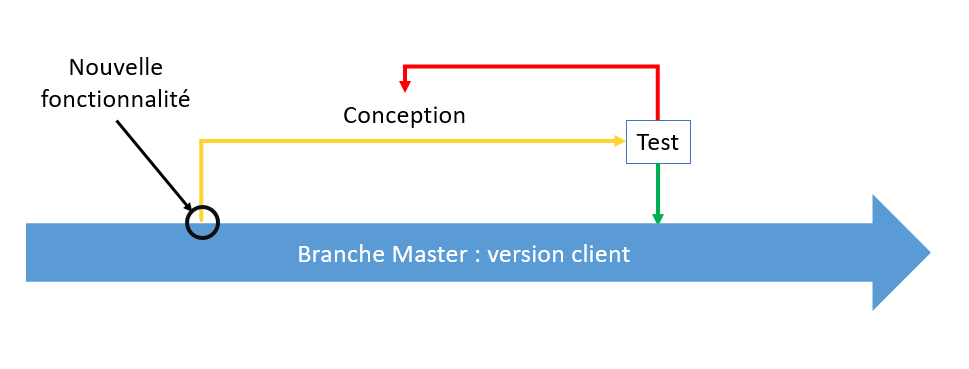
\includegraphics[width=1.0\textwidth]{images/git.PNG}
\caption{Utilisation de Git}
\label{fig:modele}
\end{figure}

\subsection{Utilisation du temps}

\paragraph{}
Pour la gestion du temps, nous avons rapidement d�velopp� toutes les classes de donn�es, les fonctionnalit�s principales et une IHM simplifi�e.
Cela nous a permis d'avoir rapidement une base de tests solide pour d�velopper les fonctionnalit�s plus complexes et une meilleure IHM.
Ensuite nous avons gard� un ryhtme constant pour ne pas prendre de retard.

\begin{figure}[H]
\centering
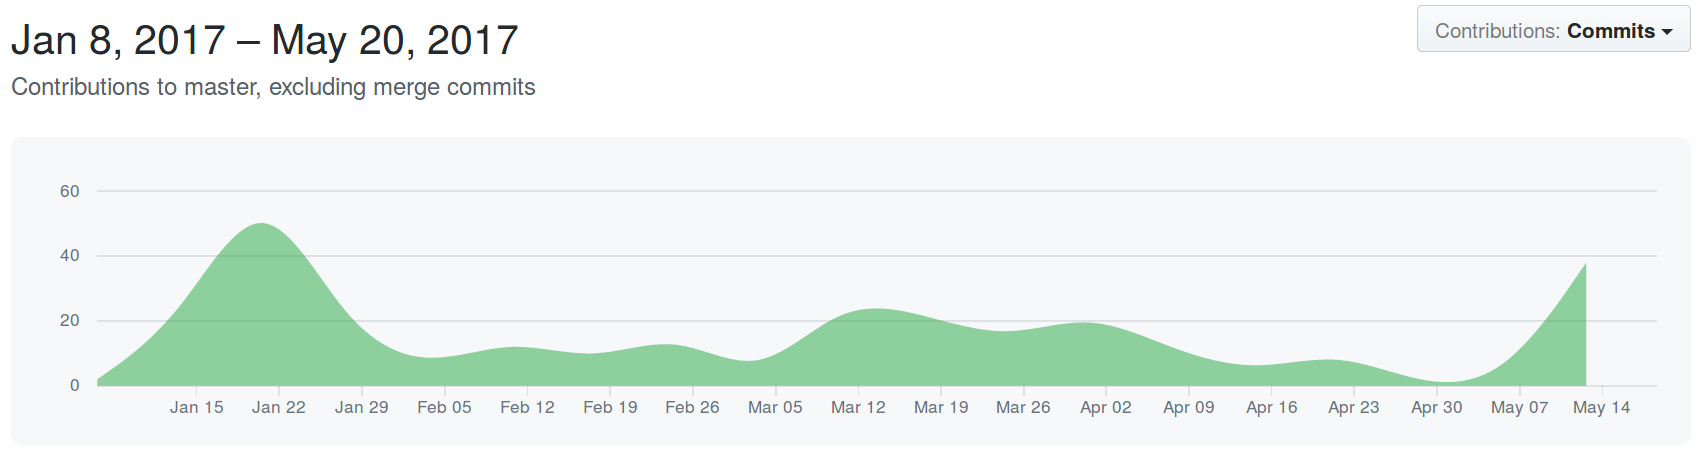
\includegraphics[width=1.0\textwidth]{images/temps.png}
\caption{R�partition des commits Git au cours du temps}
\label{fig:modele}
\end{figure}


